
%%%%%%%%%%%%%%%%%%%%%%% file typeinst.tex %%%%%%%%%%%%%%%%%%%%%%%%%
%
% This is the LaTeX source for the instructions to authors using
% the LaTeX document class 'llncs.cls' for contributions to
% the Lecture Notes in Computer Sciences series.
% http://www.springer.com/lncs       Springer Heidelberg 2006/05/04
%
% It may be used as a template for your own input - copy it
% to a new file with a new name and use it as the basis
% for your article.
%
% NB: the document class 'llncs' has its own and detailed documentation, see
% ftp://ftp.springer.de/data/pubftp/pub/tex/latex/llncs/latex2e/llncsdoc.pdf
%
%%%%%%%%%%%%%%%%%%%%%%%%%%%%%%%%%%%%%%%%%%%%%%%%%%%%%%%%%%%%%%%%%%%


\documentclass[runningheads,a4paper]{llncs}


\usepackage{amssymb,graphicx,times,amsmath,url}
\setcounter{tocdepth}{3}
\usepackage[latin1]{inputenc}
\usepackage{multirow}


\newcommand{\Prob}{\mbox{\bf P}}

\DeclareMathOperator*{\argmax}{arg\,max}

\urldef{\mailsa}\path|craf@cin.ufpe.br|
\urldef{\mailsb}\path|fatc@cin.ufpe.br|
\urldef{\mailsc}\path|igcf@cin.ufpe.br|

\newcommand{\keywords}[1]{\par\addvspace\baselineskip
\noindent\keywordname\enspace\ignorespaces#1}

\begin{document}

\mainmatter  % start of an individual contribution

%
% paper title
% can use linebreaks \\ within to get better formatting as desired

\title{Semi-supervised Approach for Finding Cancer Sub-Classes on Gene Expression Data}

% a short form should be given in case it is too long for the running head
\titlerunning{Semi-supervised Approach for Finding Cancer Sub-Classes}

% the name(s) of the author(s) follow(s) next
%
% NB: Chinese authors should write their first names(s) in front of
% their surnames. This ensures that the names appear correctly in
% the running heads and the author index.
%
\author{Clerton Ribeiro$^1$ \and Francisco de Assis T. de Carvalho$^1$ \and \\ Ivan G. Costa$^1$}
%
\authorrunning{Clerton Ribeiro et al.}
% (feature abused for this document to repeat the title also on left hand pages)

% the affiliations are given next; don't give your e-mail address
% unless you accept that it will be published
\institute{$^1$Center of Informatics, Federal University of Pernambuco, Recife, Brazil\\
\mailsa, \mailsb, \mailsc\\
}

% make the title area
\maketitle

\begin{abstract}
  The analysis of cancer gene expression is intrinsically a
  semi-supervised problem, as one is interested in building a
  classifier for diagnosis, but also on finding new sub-classes of
  cancer. We propose here a method for Mixture Discriminant Analysis
  (MDA), which can simultaneously detect sub-classes of cancer and
  perform classification.  We evaluate the method on 10 gene
  expression data sets. MDA not only improved the classification in
  some of these data sets, as it detected some known and putative
  sub-classes of cancer.
\end{abstract}

\keywords{cancer gene expression, mixture discriminant analysis, semi-supervised learning, constraint based mixture estimation}


\section{Introduction}

The measurement of the expression of all genes of cancer patients has
made possible the development of personalized
diagnostics~\cite{Veer2008}. In this context, a standard approach is
the use of machine learning methods to build a classifier for a data
set with several healthy and cancer patients or with distinct types of
cancer~\cite{Spang2003}. Moreover, analysis on such data sets have
shown the presence of unknown sub-types of cancer by the application
of clustering methods~\cite{Alizadeh2000,Golub1999}. Such findings
have made the study of gene expression of cancer to be extremely
popular, and lead to great advances in cancer
diagnosis~\cite{Veer2008}.

These facts indicate that cancer based diagnosis is intrinsically a
semi-supervised problem~\cite{Chapelle2006}. While the studies
generating the gene expression data sets give class labelling of all
samples in the data, the frequent discovery of new sub-classes has
made the application of both supervised and unsupervised methods
routine. Therefore, a method that performs classification of cancer
types simultaneously to finding new sub-classes is extremely
desirable. By using the detected sub-classes in the classification
task, the method can better delineate class boundaries/data
distribution, therefore enhancing the overall classification
accuracy~\cite{Hastie1996}.  Moreover, the detected sub-classes,
whenever they are present in the data, are interesting candidates for
further analysis by the biomedical experts.

We propose here a semi-supervised method for estimating Mixture
Discriminant Analysis (MDA) with Gaussians distributions. MDA, which
has been initially proposed in~\cite{Hastie1996}, works by fitting a
mixture of Gaussian distributions to each class in the data set. One
major drawback of this approach is the fact that one needs to estimate
the optimal number of components in the mixtures (or sub-classes) for
each class independently. This makes the method computationally costly
and requires the application of model selection procedures.  We
propose here the use of a constraint-based-mixture
estimation~\cite{Lange2005} for estimating the MDA. The method has as
input the list all negative pairwise constraints, i.e. all pairs of
patients that should not be in the same class. The algorithm, which is
based on an extension of the Expectation-Maximization (EM) algorithm,
searches for solutions with a pre-determined number of groups $K$
satisfying all negative constraints. That is, we do not have patients
of distinct classes in a single group, but we allow patients from the
same class to belong to several groups. Therefore, if $K$ is higher
than the number $C$ of classes (cancer types), the method will return
a classifier with $K-C$ novel sub-classes.

A similar approach has been previously shown to work on the
classification of time-series of Multiple Sclerosis
patients~\cite{Costa2009a}. In this work, we evaluate the MDA method
with several data sets from a cancer gene expression
compendium~\cite{Souto2008}. Furthermore, we apply a Quadratic
Discriminant Analysis (QDA), which is equivalent to MDA when $K=C$, to
serve as a baseline case.  To select the optimal number of sub-classes
$K-C$, we use a cross-validation procedure. Finally, apply a consensus
method proposed in~\cite{Monti2003} to evaluate if the sub-classes
found are stable over distinct solutions obtained by the
cross-validation procedure.

%This paper is organized as follows ...

\section{Material and Methods}

\subsection{Data Sets}


We use in this study 10 public micro-array data sets with cancer gene
expression {\small
(\url{http://algorithmics.molgen.mpg.de/Supplements/CompCancer})}. An
overview of these 10 datasets is presented in Table~\ref{dataset}.


\begin{table*}[htp]
\caption{Data set description \label{dataset}}
\begin{center}
\begin{footnotesize}
\begin{tabular}{|l|l|l|l|l|}
 \hline \bf{Dataset} & \bf{Classes} & \bf{$n$} &\bf{$C$} & \bf{$d$} \\
 \hline 
{\tt Alizadeh-v2} & DLBCL(42), FL(9), CLL(11) & 62 &3 & 4022
 \\
{\tt Alizadeh-v3}           & DLBCL1(21), DLBCL2(21), FL(9), CLL(11)      	&62		    	&4            	&4022 		\\ 
{\tt Armstrong-v1} 			& ALL(24),MLL(48)				& 72        	&2       		& 12582    \\
{\tt Armstrong-v2} 			& ALL(24), MLL(20), AML(28)		& 72    		&3       		& 12582    \\
{\tt Chen}         			& HCC(104), liver(75)			& 179         	&2       		& 22699         \\
{\tt Golub-v1}     			& ALL(47), AML(25)				& 72         	&2       		& 7129  \\
{\tt Golub-v2}     			& ALL-B(38), ALL-T(9), AML(25)	& 72         	&3       		& 7129         	\\
{\tt Nutt-v2}      			& CG(14), NG(14)   	 			& 28         	&2       		& 12625 \\
{\tt Nutt-v3}      			& CO(7), NO(15)      			& 22          	&2       		& 12625         \\
{\tt Yeoh-v1}      			& T-ALL(43), B-ALL(205)			& 248         	&2       		& 12625        	\\
\hline
\end{tabular}
\end{footnotesize}
\end{center}
\end{table*}

In Table~\ref{dataset}, the second column describes the names of the
classes (cancer types), as defined in the original publication, and
the number of samples (patients) in each class. For further
description of classes see~\cite{Souto2008}. The third column presents
the number of samples ($n$), the fourth column the number of classes
and the last column the number of genes ($d$). It is quite noticeable
from the table that all data sets are sparse with a few samples on a
high dimensional space.

The data were pre-processed by the application of an unsupervised
filter to discard missing values and genes displaying no differential
expression, as described in~\cite{Souto2008}. The pre-processing
performed on data from experiments based on the Affymetrix platform
(Alizadeh, Golub, Nutt and Yeoh) has the following steps: (1) all
values below 10 and above 16000 were replaced by these bounds,(2) we
measured the mean expression of each gene and eliminate 10$\%$ of the
highest and lowest values to avoid extreme values (3) each expression
value was replaced by the base 2 log transformation of the ratio
between the expression value and the gene mean expression. For cDNA
platform data (Armstrong and Chen), it was not necessary to apply
transformations, as they were already in logarithmic scale. The
unsupervised filter process was as follows: two $l$ and $c$ thresholds
were chosen, where the absolute value of the feature has to be higher
than $l$ in at least $c$ patients. Genes that do not fit this
restriction were excluded from the data set. 

%For data measured with
%the Affymetrix micro-arrays, which give counts as estimated of
%expression, we applied a log transformation in order to make the
%distribution closer to Gaussian.

\subsection{Classification Algorithms}

Let $X$ be a $d$ by $n$ matrix representing a gene expression data
set, where $x_{ij}$ denotes the expression value of sample (patient)
$j$ and feature (gene) $i$, $x_i$ is a $d$-dimensional vector with the
expression values of sample (patient) $i$. We also have associated to
each data set a vector $Y$ with dimension $n$, where $y_i \in \{1,...,C\}$
denotes the class sample $i$ belongs to.

\subsection{Discriminant Analysis}

Discriminant analysis (DA) methods perform classification by inference
over the posterior distribution $\Prob[y|x]$~\cite{Hastie2001}. Let
$\Prob[x_i|y_i=c]$ be the class-conditional density modeling the
distribution of samples in class $c$ and $\pi_c$ be the prior
distribution of class $c$, such that $\sum_{c=1}^C \pi_c =1$ and
$\pi_c \geq 0$, we can use Bayes Theorem to derive the posterior
probability
\begin{equation}
\label{eq:classcond}
\Prob[y_i=c|x_i] = \frac{\pi_c \Prob[x_i|y_i=c]}{\sum_{c'=1}^C \pi_{c'} \Prob[x_i|y_i=c']}.
\end{equation}
Therefore, classification of a sample $x_i$ can be performed with the
rule
\begin{equation}
\hat{y_i} = \argmax_{c=\{1,...,C\}} \Prob[y_i=c|x_i].
\label{eq:class}
\end{equation}
as given in Eq.~\ref{eq:class}, where $\hat{y_i}$ is the predicted class for sample $i$.

The definition of $\Prob[x_i|y_i=c]$ is application dependent.  In
gene expression analysis, a usual choice is a multivariate Gaussian
density function~\cite{Dudoit2002}, which is defined as
\begin{equation}
\label{eq:gaussian}
\Prob[x_i|y_i=c,\theta_c] = \frac{1}{\sqrt{(2\pi)^d |\Sigma_c|}} \exp^{\frac{1}{2}(x_i - \mu_c)^\mathbf{T}\Sigma_c^{-1}(x_i - \mu_c)},
\end{equation}
where $\theta_c$ are the parameters $(\mu_c,\Sigma_c)$. $\mu_c$ and
$\Sigma_c$ can be estimated with the mean and covariance matrices of
samples of class $c$ and $\pi_c=n_c/n$, where $n_c$ is the number of samples
in class $c$~\cite{Hastie2001}.

Given sparsity of the data (few samples and high dimension), it is
usual to assume independence among the attributes given the class.
In gene expression analysis this is done by estimating a diagonal
parameterization of the covariance matrix $\Sigma_c$, i.e.  only the
diagonal entries are estimated and all other values are set to
zero~\cite{Dudoit2002}. This variant of DA is known as Diagonal
Quadratic Discriminant Analysis (DQDA) and will be used in this study
as a baseline method.

\subsection{Mixture Discriminant Analysis}

With mixture of discriminant analysis (MDA), we assume that class
condition densities can be defined as a mixture model, that is
\begin{equation}
\label{eq:mixture}
\Prob[x_i|y_i=c] = \sum_{k=1}^K \alpha_k \Prob[x_i|z_i=k],
\end{equation}
where $\alpha_k,i=1,...,K$ are the mixing coefficients.
In~\cite{Hastie1996}, the estimation of these mixture were performed
with the application of the EM algorithm for each class to be
classified. 


\subsection{Mixture Model Estimation with Constraints\label{sc:mmec}}

A standard mixture model can be defined as 
\begin{equation}
\label{eq:density}
\Prob[x_i|\Theta] = \sum_{k=1}^K \alpha_k \Prob[x_i|y_i=k,\theta_k]
\end{equation}
as given in Eq.~\ref{eq:density},where $\Theta = (\alpha_1, ..., \alpha_k, \theta_1, ..., \theta_K)$
are the model parameters and $\alpha_k$ are the mixing coefficients.
By including a set of hidden labels represented by the $n$-dimensional
vector $Z$, where $z_i
\in \{1,..,K\}$ defines the component generating the $x_i$, we obtain
the complete data likelihood
\begin{equation}
\label{eq:likelihood}
\Prob[X,Y|\Theta] = \Prob[X|Z,\Theta] \Prob[Z|\Theta].
\end{equation}
We can use then the {\tt EM} method to estimate the parameters
$\Theta$ and component assignments $Z$ maximizing the complete
likelihood (see~\cite{MacLachlan2000} for details).

In constrained-based-mixture estimation (and its similar constrained
based clustering), the user can define a $n \times n$ matrix $W$ with
negative pairwise constraints, where $w^-_{ij}=1$ if samples $i$ and
$j$ should not belong to the same mixture component and $w^-_{ij}=0$
otherwise. The constraints are incorporated in the estimation by
extending the prior probability of the hidden variable to
$\Prob[Z|\Theta,W]=\Prob[Z|\Theta]\Prob[W|Z]$. Assuming $\Prob[W|Z]$
follows a Gibbs distribution, there is a variation of the EM algorithm
for estimating $Z$ and $\Theta$~\cite{Lange2005,Lu2005}. The method
requires the redefinition of the posterior assignment distribution as
\begin{equation}
%\mbox{\small{$
\Prob[z_i=k|x_i,W] = \frac{\pi_c \Prob[x_i|z_i=k]}{\mathcal{Z}} \exp^{\sum_{j \neq i} -\lambda^- w^-_{ij} \Prob[z_j=k|x_j,W]},
%$}}
\label{eq:posterior}
\end{equation}
where $\mathcal{Z}=\sum_{k=1}^K\Prob[z_i=k|x_i,W]$ and $\lambda^-$ is
the Lagrange parameter defining the penalty weight of constraints
violations.

\subsection{Constraint-based Mixture Discriminant Analysis}

We propose here the use of the constraint-based mixture estimation
method described above for obtaining a MDA classifier. By setting the
penalty parameter $\lambda^-$ with a high value and the constraint
matrix $W$, such that $w^-_{ij}=1$ if $y_i \neq y_j$ and $w^-_{ij}=0$
otherwise, we will obtain solutions where samples with distinct
classes are not in the same mixture component. Furthermore, by
choosing a number of components $K>C$, some of the classes will be
related to more than one mixture component. In other words, the
mixture will divide some of the classes in sub-classes.

Therefore, we need a procedure to relate the mixture components with
the classes.  This can be achieved by relating the assignment vector
$Z$ of the mixture with the class vector $Y$. We can estimate the
probability of obtaining class $c$ given component $k$ by
\begin{equation}
\Prob[y=c|z=k]=\frac{\sum_{i=1}^N \mathbf{1}(y_i=c) \mathbf{1}(z_i=k)}{\sum_{i=1}^N \mathbf{1}(z_i=k)},
\label{eq:component}
\end{equation}
where $\mathbf{1}$ is the identity function. From this, we can define
the mapping
\begin{equation}  
\mbox{ClassOf}(k) =\argmax_{c=\{1,...,C\}} \Prob[y=c|z=k],
\label{eq:classcomponent}
\end{equation}
which defines the class $c$ related to component $k$. 

We can use this mapping and parameters $\Theta$, which has been
estimated with the method described in Section~\ref{sc:mmec}, to define
the class conditionals as defined in Eq.~\ref{eq:mixture} and obtain a
MDA classifier with the use of Eq.~\ref{eq:classcond}.


\subsection{Experimental Design and Consensus Analysis}

For each data set, we performed a leave-one-out cross-validation. All
accuracies described in the following are based on the test set alone.
Then we use the Friedman test followed by a multiple comparison
correction procedure to access the significance of the ranking of the
methods~\cite{Dem2006}. For the final interpretation of the
sub-classes, we need a method for combining the results of the
classifiers (training and test sets) for all leave one out runs.  For
this task, we use a procedure proposed in~\cite{Brunet2004,Monti2003}.  First, we
build a co-occurrence matrix by counting for each pair of samples the
number of times they appear in the same component across the different
solutions $Z$. The consensus method works by reshuffling the matrix
and clustering samples that share similar groups over
solutions~\cite{Monti2003}.

\section{Experiments and Results \label{sec:expres}}

We investigate here if the use of the Mixture Discriminant Analysis
method improves classification accuracy in relation to the baseline
method DQDA, which is the equivalent to MDA when $K=C$. Data sets,
where the MDA improves or sustains the classification accuracy, are of
interest, as these indicate the presence of sub-classes of cancer.

\begin{table}[htp]
\caption{Accuracy and standard deviation from classification methods for each data set \label{results}}
\begin{center}
\begin{footnotesize}
\begin{tabular}{|l|c|c|c|}
  \hline
  \bf{Dataset}     & DQDA    & MDA $c+1$  & MDA $c+2$  \\
  \hline
  {\tt Alizadeh-v1}  & \textbf{95.24} (21.55) 	& 80.95 (39.74)  	& 80.95 (26.07) \\  
  {\tt Alizadeh-v2}  & 96.77 (17.81)   			& \textbf{100} (0) 	& \textbf{100} (0) \\  
  {\tt Armstrong-v1} & 98.61 (11.79)			& 97.22 (16.55)  	& 98.61 (11.79) \\           
  {\tt Armstrong-v2} & \bf{94.44} (23.07) &\bf{94.44} (23.07) & 88.89 (11.79)       \\    
  {\tt Chen}         & 91.62 (27.79)	& 91.06 (28.61)	& 94.41 (20.72)       \\
  {\tt Golub-v1}   & \bf{98.61} (11.79) & 97.22 (16.55)	& 93.05 (16.55)        \\
 {\tt Golub-v2}     & 90.28 (29.83) & 90.27 (29.83)  & 90.27 (20.12)        \\           
 {\tt Nutt-v2} 		& 78.57 (41.79)	& 71.42 (46.00)  & 82.14 (31.50)        \\      
 {\tt Nutt-v3}      & 86.36 (35.13) & 90.9 (29.42) & 81.81 (38.56)        \\             
 {\tt Yeoh-v1}      & \bf{96.16} (21.50)	& 92.74 (26.00)	& 91.93 (16.60)       \\ 
 \hline
\end{tabular}
\end{footnotesize}
\end{center}
\end{table}

We depict the accuracies and standard deviation in Table~1. Values in
bold face represent the method, which obtained a statistically
significant improvement as indicated by the Friedman
test~\cite{Dem2006}. For three datasets (Alizadeh-v1, Golub-v1 and
Yeoh-v1), DQDA obtained best results. In Alizadeth-v2 MDA with c+1 and
c+2 obtained better results and in Armstrong-v2 both DQDA and MDA c+1
were best. In all other cases, there was no statistically relevant
difference. Note that we used a leave-one-out cross-validation,
due of the small number of samples in the data sets. Such setting,
usually lead to low accuracy bias but high deviation, lowering the
statistical power of comparisons~\cite{Braga-Neto2004}.

\begin{figure*}
\centerline{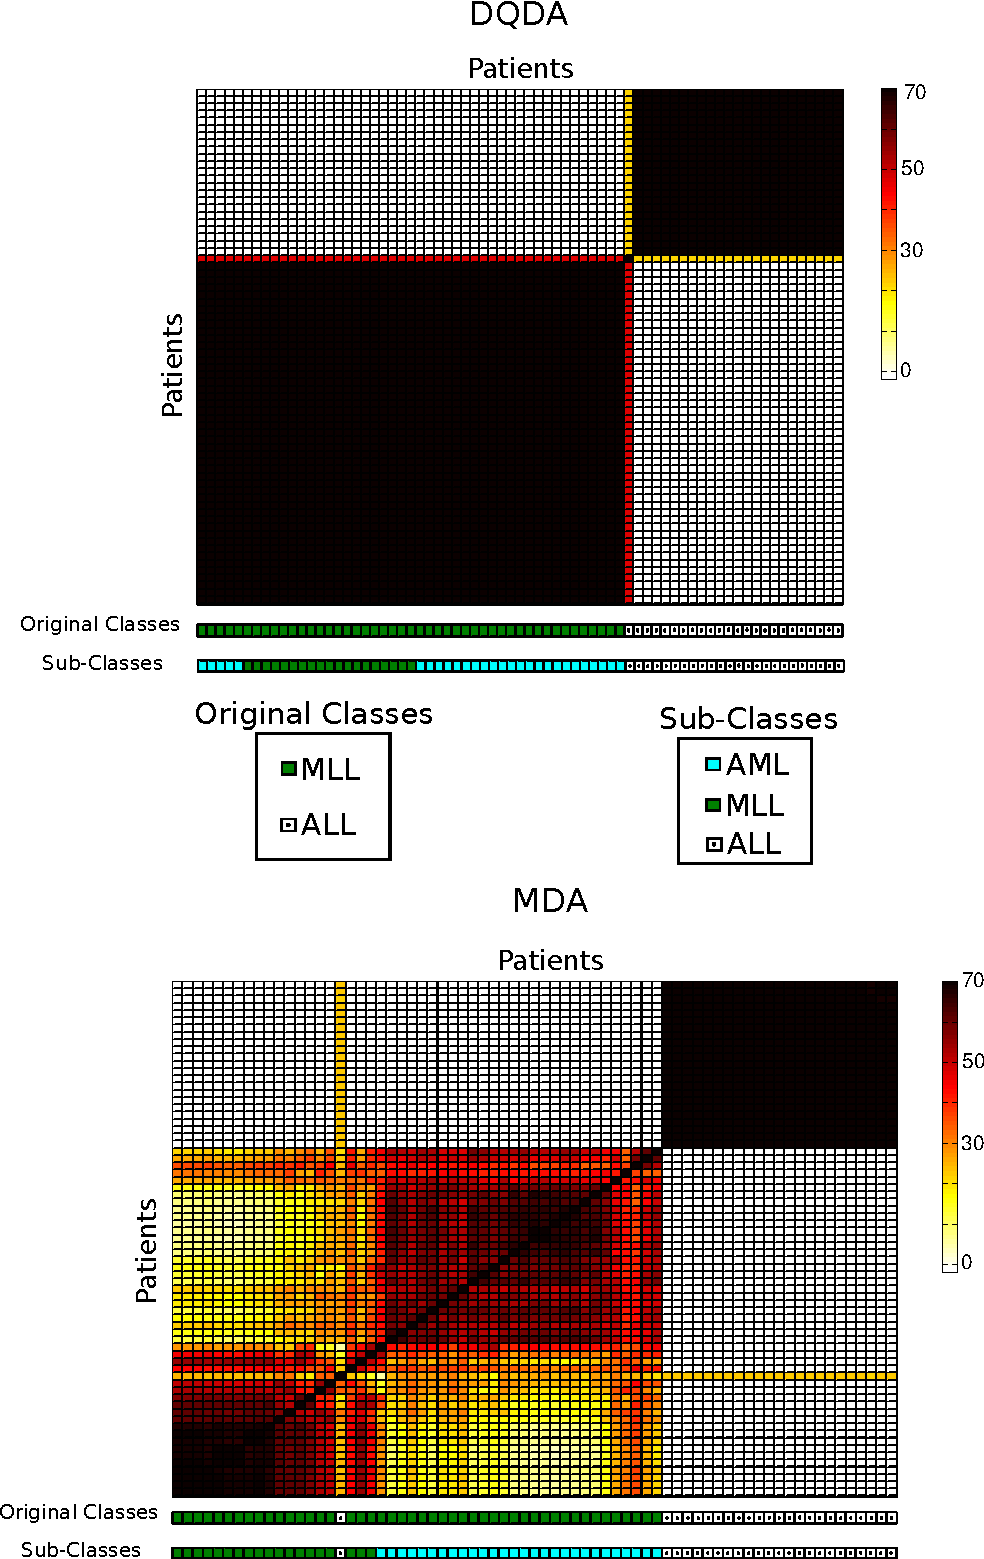
\includegraphics[width=1.0\columnwidth]{figs/DQDA_MDA2}}
\caption{Consensus Analysis on the Armstrong-v2 data for DQDA (top) and MDA $C+1$ (bottom). 
\label{fig:consensus}} 
\end{figure*}


As expected, MDA did not obtained a higher accuracy than DQDA in all
data sets, not all data sets contain sub-classes. Moreover, the
limited number of patients may lead to over-fitting with solutions
with many sub-classes (too complex models).  In some scenarios MDA was
better or equivalent to DQDA.  As the existence of sub-classes is
interesting from the application problem, we prefer the solution of
MDA with more components, whenever accuracy is equivalent to DQDA.

Some of the data sets above, Alizadeh-v1, Armstrong-v2 and Gollub-v2,
represent the original classification performed by the specialists,
which were latter found to contain sub-classes with the use of
unsupervised methods~\cite{Alizadeh2000,Armstrong2002,Golub1999}. In
these scenarios, MDA had superior or equivalent accuracies in relation
the QDA.

To assess if MDA is successful in detecting the sub-classes, we
perform the consensus analysis~\cite{Brunet2004,Monti2003} on the
Armstrong-v2 data set. In Figure~\ref{fig:consensus}, we depict the
co-occurrence matrix, where a particular entry indicates the number of
times the pair of patients were classified in the same class/sub-class
(darker values indicate higher counts). Ideally, the consensus matrix
should a block of dark values for each class indicating that the same
patients were consistently classified together. As seen in
Figure~\ref{fig:consensus} top, DQDA obtained an almost perfect
classification and separated all but one patient from the original
classes: lymphoblastic leukemias with MLL translocations (MLL) and
Acute lymphoblastic leukemias (ALL)~\cite{Armstrong2002}. This is
indicated in the figure by the two block of dark values.

The original study applied a clustering algorithm and found that 28
patients, which were originally classified as patients with MLL, had
distinct expression signatures from other MLL
patients~\cite{Armstrong2002}. These had their diagnostics changed to
akute myelogenous leukemias (AML). As indicated in
Figure~~\ref{fig:consensus} bottom, MDA with $c+1$ components,
detected the subclasses AML and MLL as indicated by the two blocks of
dark values in the left-bottom part of the matrix. Note that in this
data set, only the two original classes (MLL and ALL) were given as
input for the constraints. This exemplifies a case when MDA
successfully finds sub-classes.


%One particular data set, which has no known sub-classes, but that
%shows a slight increase with MDA c+2 in Chen.  XXX.
% XXX look at nutt-v3, singh,  - they all contaim possible sub-classes.

Another interesting data set is Nutt-v3, where we see a improvement on
the classification accuracy of MDA in relation to DQDA. Moreover, the
co-occurrence analysis indicated two sub-classes of patients with
non-classic anaplastic oligodendrogliomas, with respectively 11 and 4
patients. These non-classic gliomas are of difficult diagnosis and
these sub-classes have not been previously reported in the original
study~\cite{Nutt2003}. We detected a significant difference (t-test
with $p$-value $<$ 0.05) in the patient survival time: 672 days for
sub-class 1 and 1079 days for sub-class 2.

Next, we explored the genes (features) that are discriminative between
these sub-classes by estimating the Fisher discriminant ratio for all
genes and ranking them. We selected the 50 most discriminant genes for
each class and we performed an enrichment analysis with the g:profiler
tool~\cite{Reimand2007}.  The analysis revealed that genes
up-regulated in sub-class 1 are related to metabolic process and cell
cycle, while genes over-expressed in sub-class 2 are related to immune
response. These indicate a quite distinct expression signature of
these sub-classes, possibly as a result of distinct immune response of
the patients to cancer.  However, further patient and clinical data
are required for the validation of the potential sub-classes.

\section{Final Remarks}

We propose a new method for estimation of mixture discriminant
analysis. This methods improves the original proposal of
MDA~\cite{Hastie1996} by requiring only one pass of the EM algorithm
to obtain solutions. In the analysis of cancer gene expression, we
have shown that MDA can improve classification and successfully
indicate the existence of sub-classes of cancer of gene expression
data sets. This was exemplified on the classical study from Armstrong
et al.~\cite{Armstrong2002}. Moreover, interesting sub-classes of
non-classical gliomas were found in the Nutt data set. 

As future work, we would like to either include new data sets in the
study and perform a more detailed biological analysis of the
sub-classes found. From a methodological point of view, the MDA can be
improved by the use of feature selection methods to cope with the
high-dimensionality problem, for example using an approach similar to
Shrunken centroids~\cite{Tibshirani2002}.

% use section* for acknowledgment
\section*{Acknowledgment}

This work has been partially supported by Brazilian research agencies:
FACEPE, CNPq and CAPES.


\bibliographystyle{abbrv}
\bibliography{bases,cc}

\end{document}
